\section{Example Domains}
We apply approximate abstraction to four example domains---NChain, Taxi, Minefield and Random. These domains were selected for their diversity---NChain is relatively simple, Taxi is goal-based and hierarchical in nature, Minefield is stochastic, and Random MDP has many near-optimal policies.

% Description of visuals.
We provide visuals of both ground \acp{MDP} and resulting abstract \acp{MDP} in which a grey circle indicates a state and colored arrows indicate transitions. The thickness of the arrow indicates how much reward is associated with that transition. In the ground \acp{MDP}, states are labeled with a number. In the abstract \acp{MDP}, we indicate which ground states were collapsed to each abstract state by labelling the abstract states with their ground states. %(some are visually unwieldy and so were not labelled).

%Description of code base
Our code base (link redacted for review) provides implementations for abstracting arbitrary \acp{MDP} as well as visualizing and evaluating the resulting abstract \acp{MDP}. We use the graph-visualization library GraphStream~\cite{graphstream} and the planning and \ac{RL} library, BURLAP~\cite{BURLAPCITATION}.

% Subsection: NChain.
\subsection{NChain}

NChain, pictured in Figure~\ref{fig:nchain-visual}, is a simple MDP heavily investigated in the Bayesian RL literature due to the interesting exploration problem it poses~\cite{dearden1998bayesian}. In all states, the agent has two actions available: advance down the chain, or return to state 0. The agent receives a small positive reward, $r_{small}$ for returning to state 0, and no reward for advancing down the chain. The exception is that when the agent transitions to the last state in the chain, it receives a large positive reward, $r_{large}$. Transitions also have small slip probability $\rho$, such that the applied action results in the opposite dynamics. In our implementation, we set $N=10$, $\rho=0.2$, $r_{small} = 0.2$, and $r_{large} = 1.0$.

% NChain Compression Visuals.
\begin{figure}[h]
\subfigure[Ground NChain]{
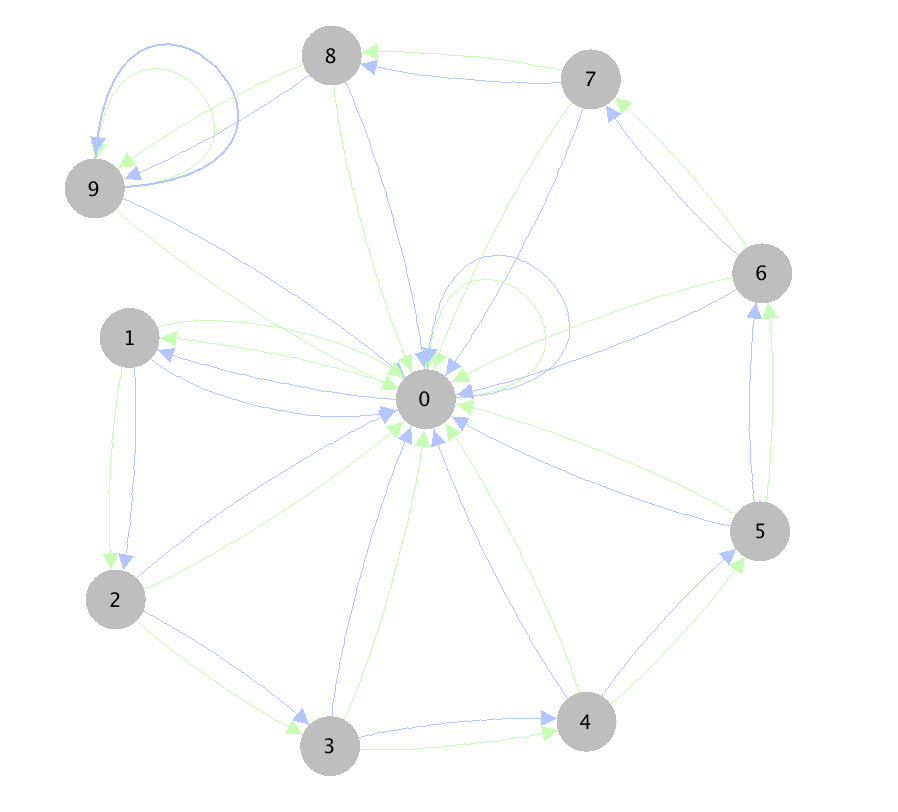
\includegraphics[width=0.48\columnwidth]{figures/ground_nchain.png}}
\subfigure[Abstract NChain]{
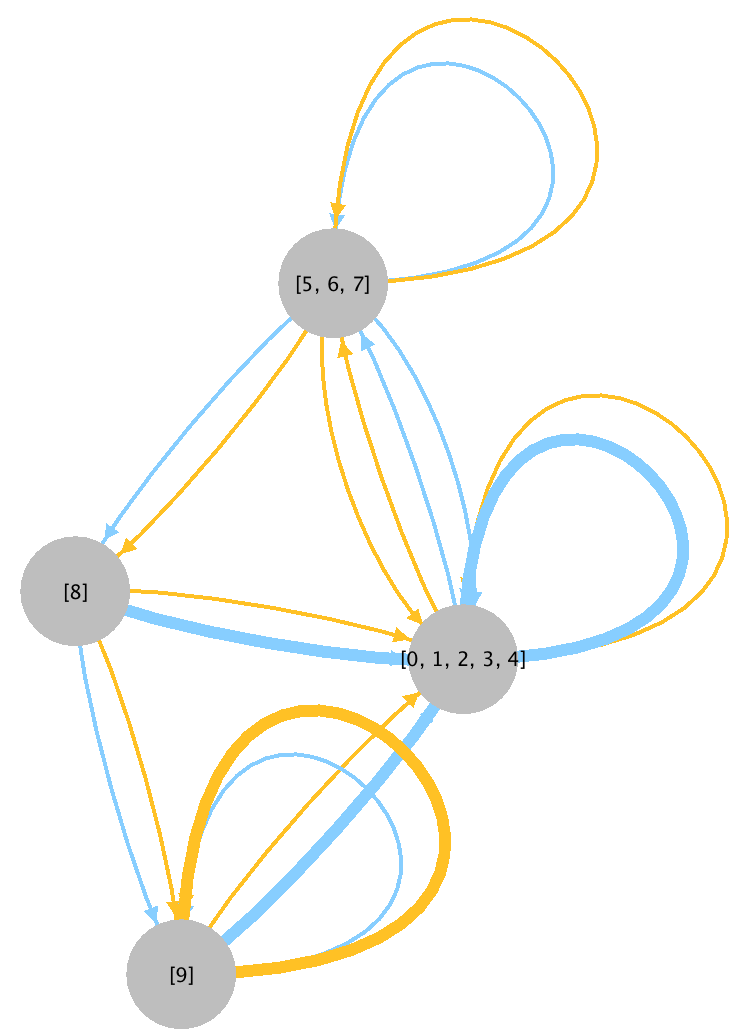
\includegraphics[width=0.48\columnwidth]{figures/abs_nchain.png}}
\label{fig:nchain-visual}
\caption{Comparison of ground NChain \ac{MDP} and abstract NChain \ac{MDP}, under an $\epQ$ abstraction, with $\epsilon=0.5$}
\end{figure} 

%% Subsection: UpWorld.
%\subsection{UpWorld}
%
%The UpWorld task is an $N\times M$ grid in which the agent starts in the lower left corner. The agent may move left, right, and up. The agent receives positive reward for transitioning to a state at the top of the grid, where moving up in the top cells self transitions. the agent receives 0 reward for all other transitions. Consequently, moving up is always the optimal action, since moving left and right does not change the agent's manhattan distance to positive reward. During experimentation, we set $N=10$, $M=4$.
%
%\begin{figure}
%\subfigure[Ground UpWorld]{
%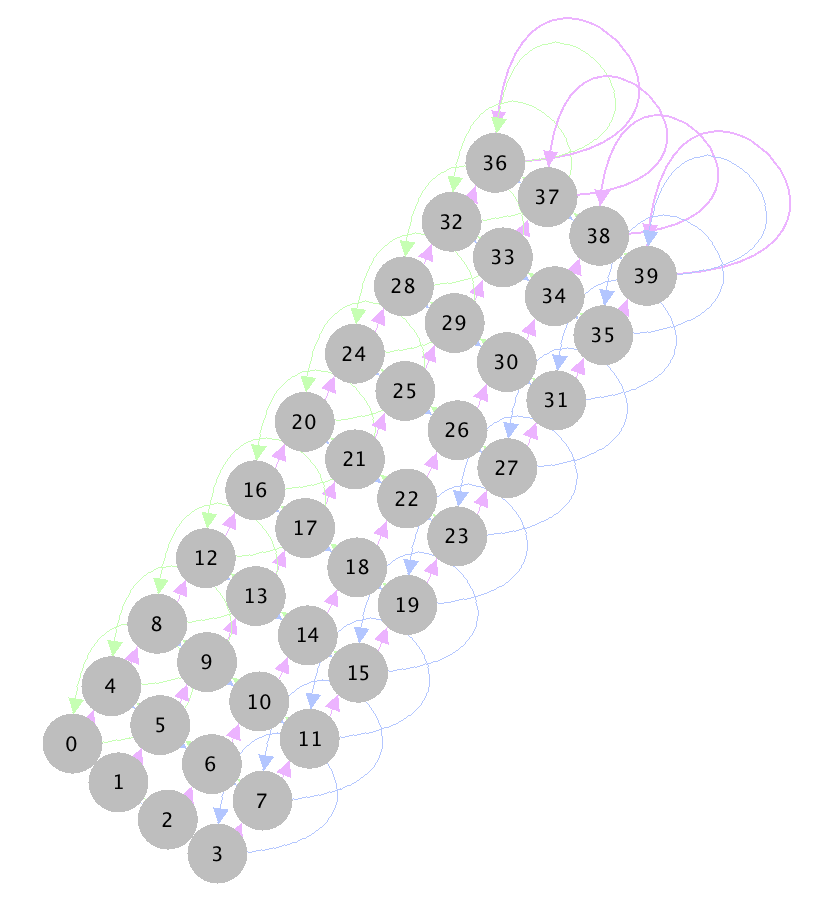
\includegraphics[width=0.48\columnwidth]{figures/ground_upworld.png}}
%\subfigure[Abstract UpWorld]{
%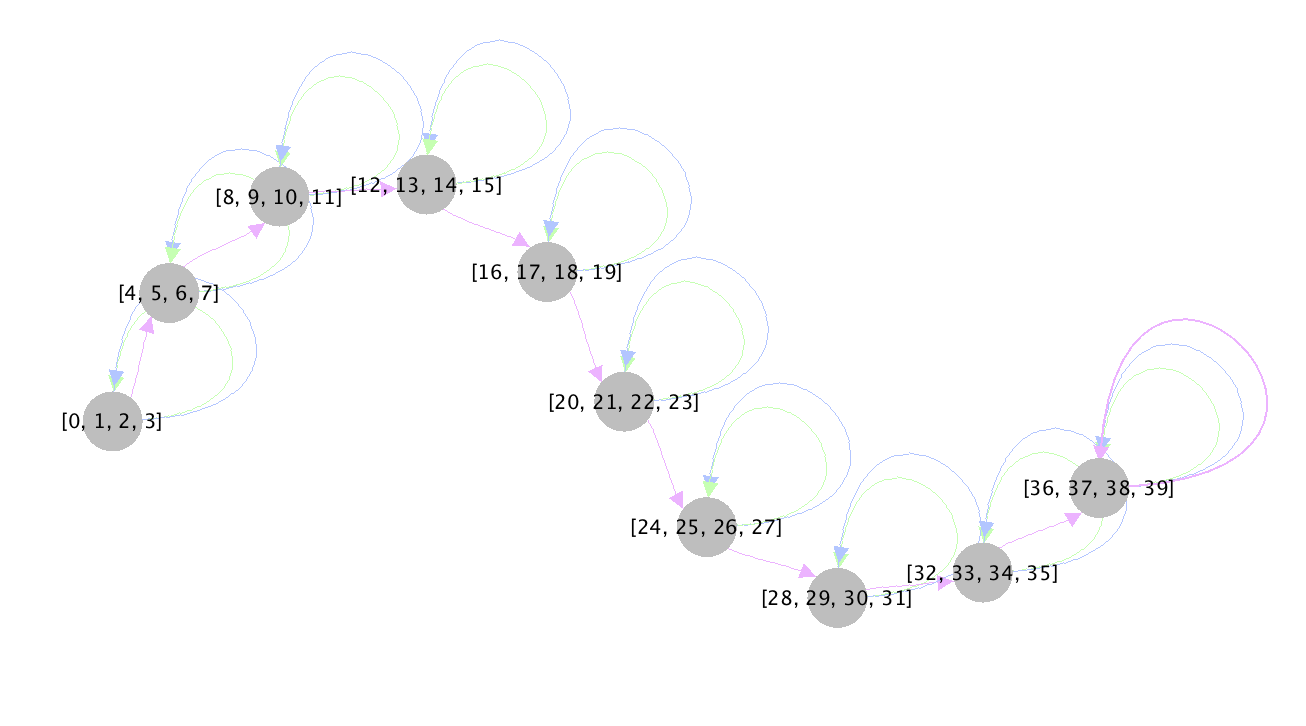
\includegraphics[width=0.48\columnwidth]{figures/abs_upworld.png}}
%\label{fig:upworld-visual}
%\caption{Comparison of Original UpWorld MDP and Abstract MDP, under $\epQ$, with $\epsilon=0.5$}
%\end{figure} 

% Subsection: Taxi
\subsection{Taxi}

Taxi has long been studied by the hierarchical RL literature~\cite{dietterich2000hierarchical}. The agent, operating in a grid-world style domain, may move left, right, up, and down, as well as pick up a passenger and drop off a passenger. The goal is achieved when the agent has taken all passengers to their destinations.

%We visualize the compression on a simple 626 Taxi instance in Figure~\ref{fig:taxi-visual}. As stated above, we visualize the original Taxi problem into a graph representation so that we may visualize both the ground MDP and abstract MDP in the same format.

% Taxi Compression Visuals
%\begin{figure}[h]
%\subfigure[Ground Taxi]{
%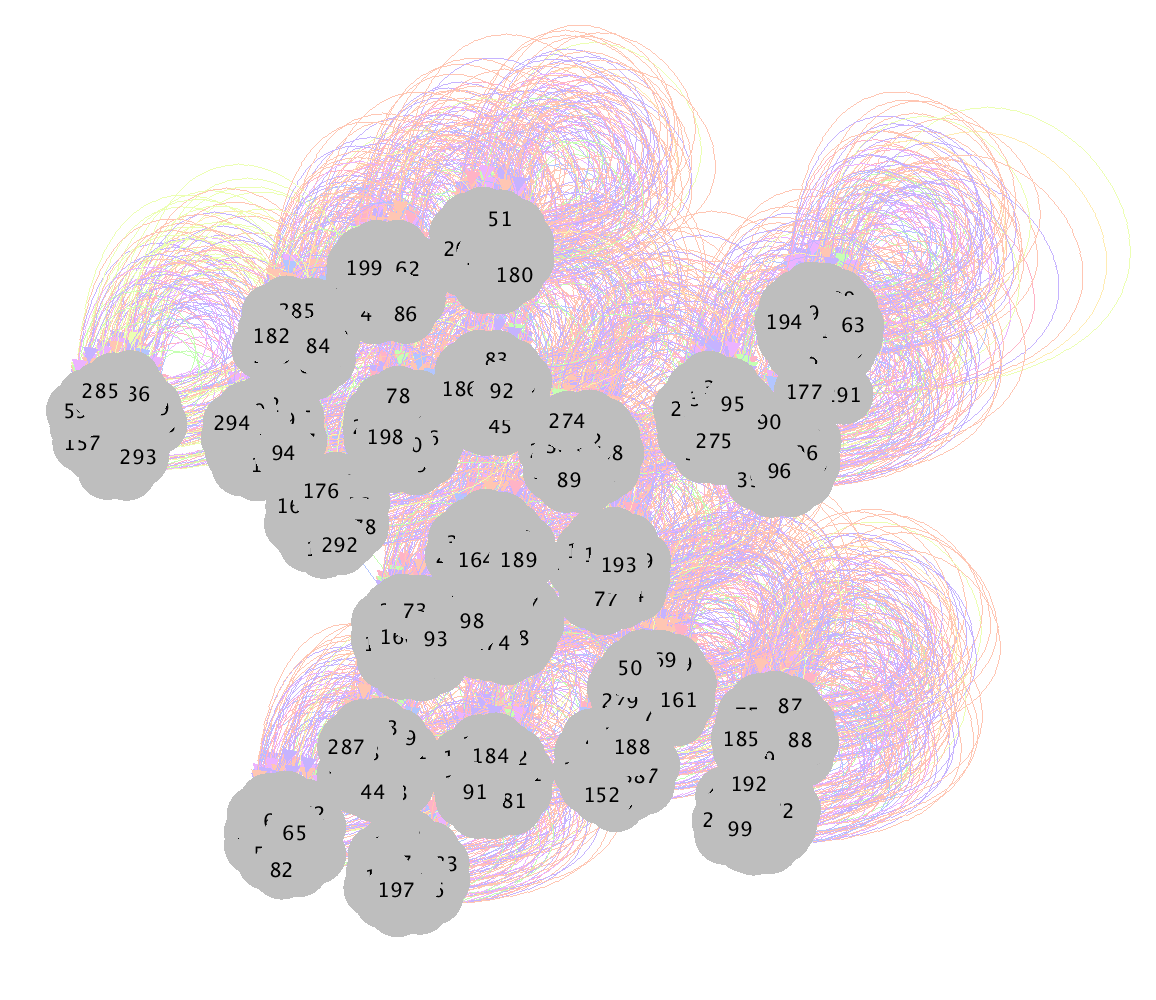
\includegraphics[width=0.48\columnwidth]{figures/ground_taxi.png}}
%\subfigure[Abstract Taxi]{
%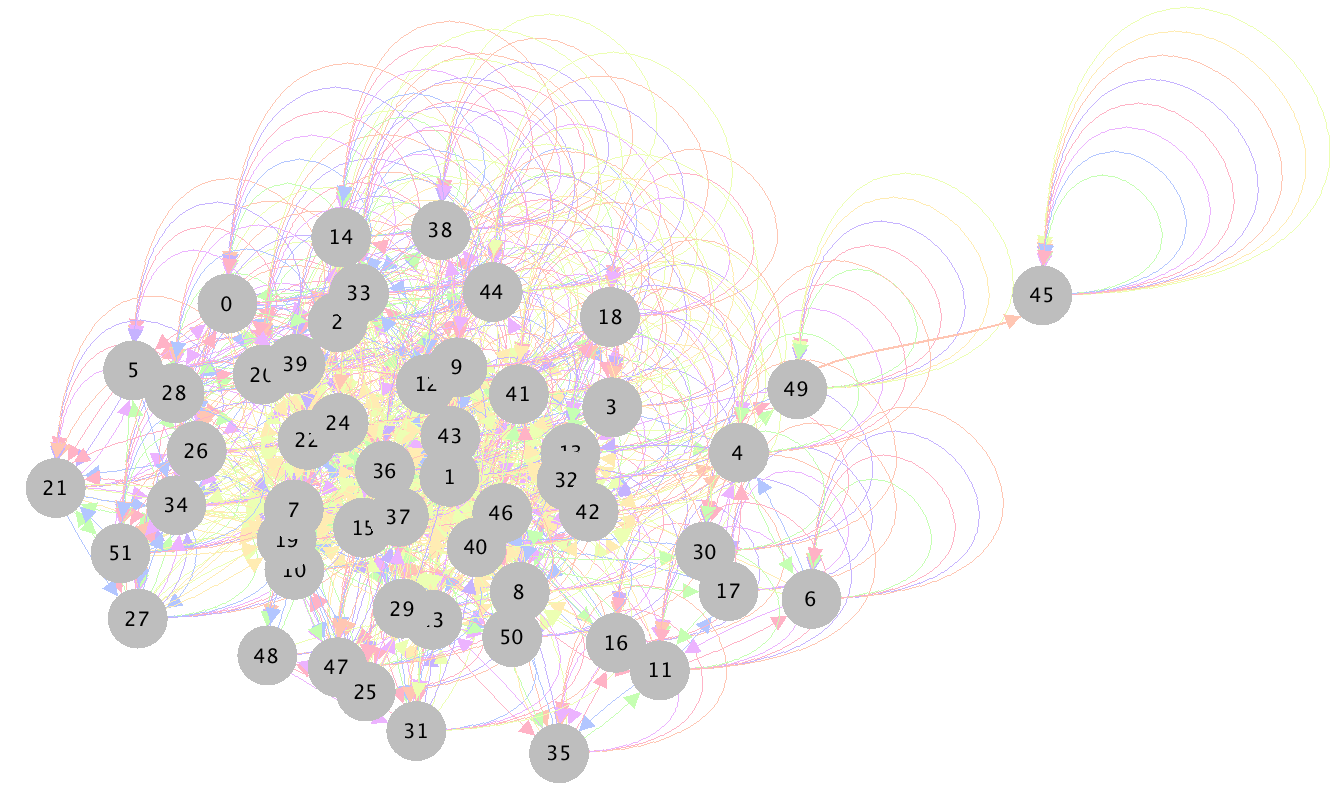
\includegraphics[width=0.48\columnwidth]{figures/abs_taxi.png}}
%\label{fig:taxi-visual}
%\caption{Comparison of Original Taxi MDP and Abstract Taxi MDP, under an $\epQ$ abstraction, with $\epsilon=0.03$}
%\end{figure} 


% Insert visual and/or stats on number of states and performance of VI solving the abstract MDP and evaluating the resulting policy on the original MDP


% Subsection: Minefield.
\subsection{Minefield}

Minefield is a test problem we are introducing that uses the Grid World dynamics of \citeauthor{russell1995modern} with slip probability of $x$. The reward function is such that moving up in the top row of the grid receives $1.0$ reward; all other transitions receive $0.2$ reward, except for transitions to a random set of $\kappa$ states (which may include the top row) that receive $0$ reward. (These are the states with ``mines'' in them.) We set $N=10, M=4, \epsilon=1.1, \kappa = 5, x = 0.01$. We depict the original Minefield and an abstract Minefield in Figure~\ref{fig:minefield-visual}.

zzz problem: text says ``top row'', but image is oriented diagonally.

% Minefield Compression Visuals
\begin{figure}
\subfigure[Ground Minefield]{
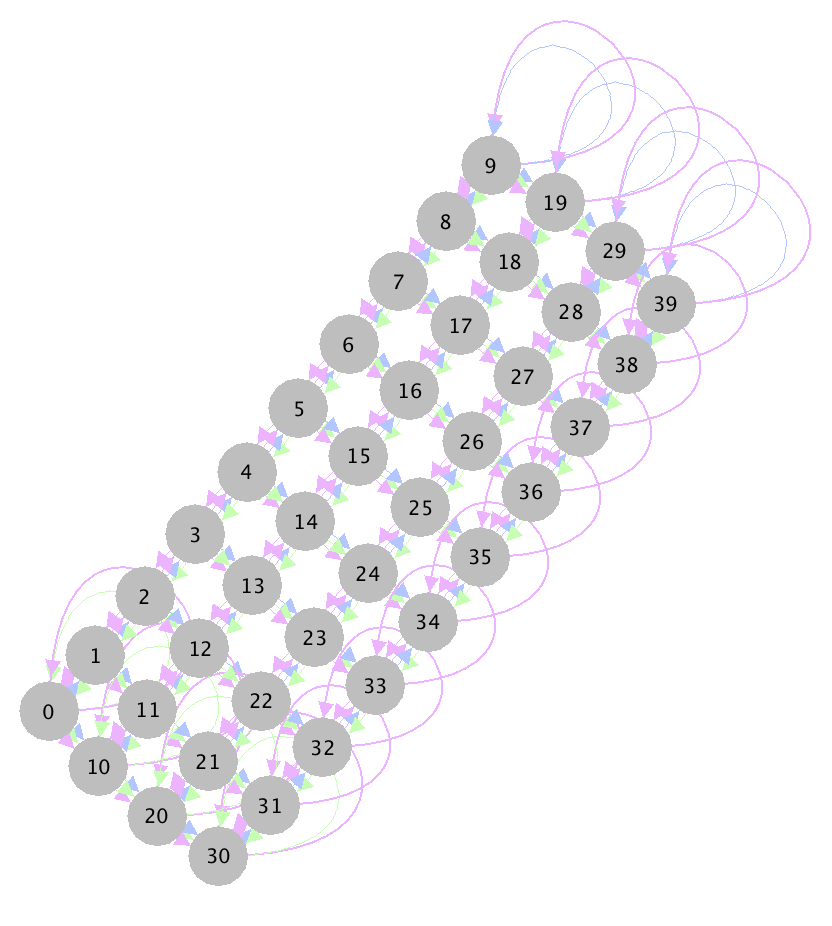
\includegraphics[width=0.48\columnwidth]{figures/ground_minefield.png}}
\subfigure[Abstract Minefield]{
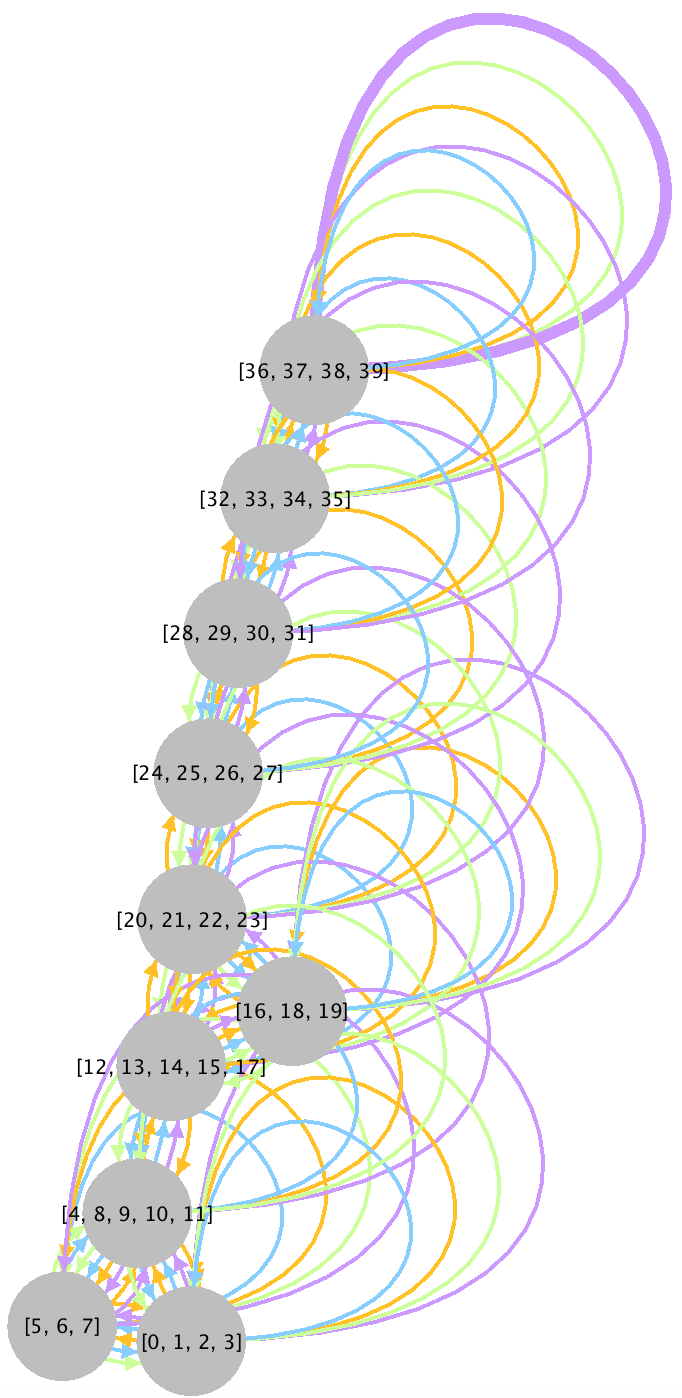
\includegraphics[width=0.48\columnwidth]{figures/abs_minefield.png}}
\label{fig:minefield-visual}
\caption{Comparison of ground Minefield \ac{MDP} and abstract \ac{MDP}, under a $\epQ$ abstraction with $\epsilon=1.1$}
\end{figure} 
zzz the lines are very thin... not visible to me.

% Subsection: Random.
\subsection{Random}

In the Random \ac{MDP} domain we consider, there are $N$ states and $K$ actions. For each state, each action transitions to one of two randomly selected states, each with probability $0.5$.

%The Random MDP and its compression are visualized in Figure~\ref{fig:minefield-visual}.

% Random Compression Visuals
%\begin{figure}
%\subfigure[Ground Random]{
%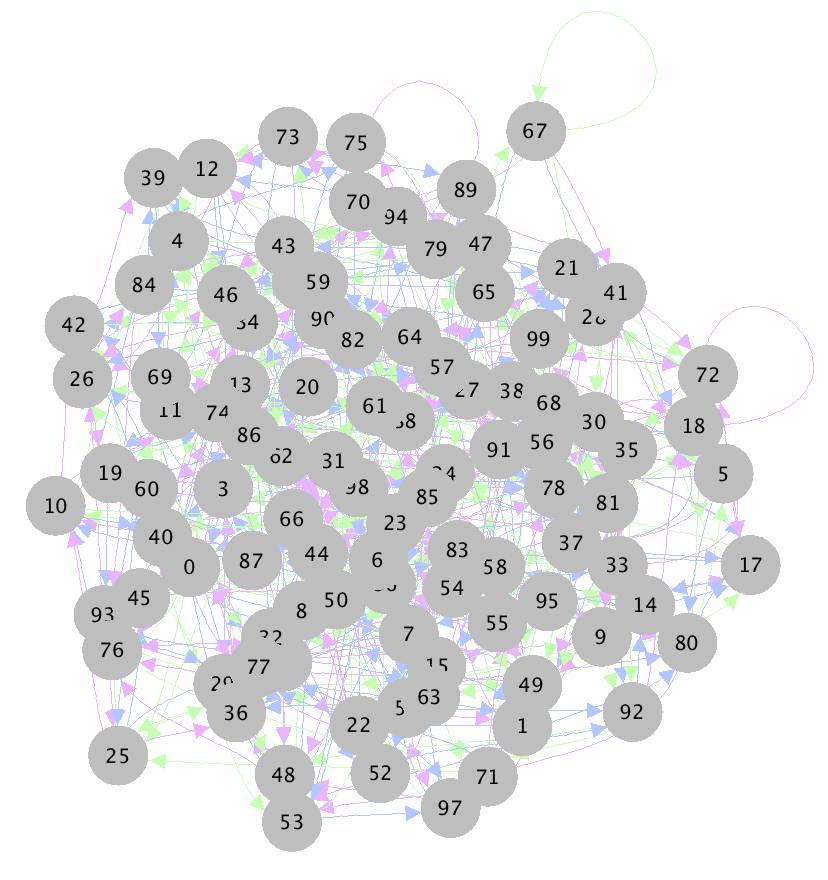
\includegraphics[width=0.48\columnwidth]{figures/ground_random.png}}
%\subfigure[Abstract Random]{
%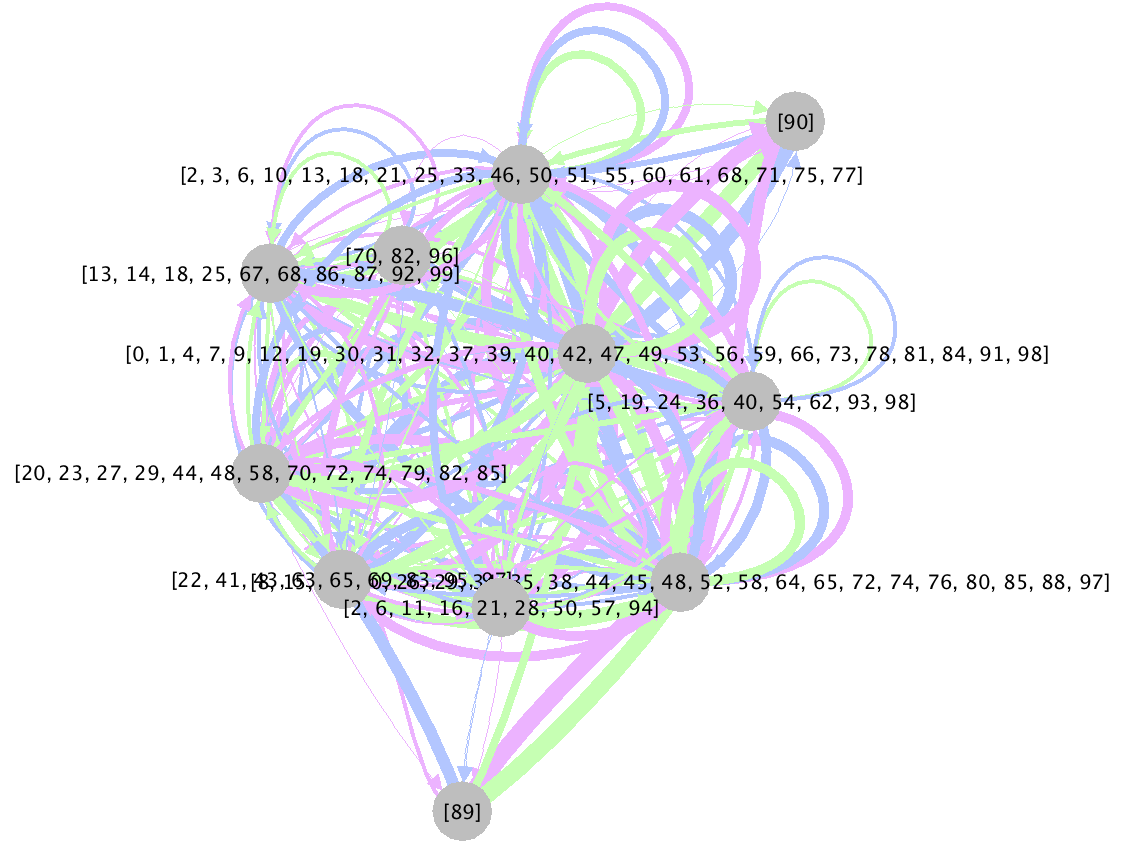
\includegraphics[width=0.48\columnwidth]{figures/abs_random.png}}
%\label{fig:minefield-visual}
%\caption{Comparison of Original Random MDP and Abstract Random MDP, under an $\epQ$ abstraction, with $\epsilon=0.2$}
%\end{figure} 
